%!TEX root = thesis.tex

\chapter{Scalable Music Tagging with Poisson Factorization}\label{chpt:tagging}

%\begin{abstract}
Automatic music tagging is an important but challenging problem within \gls{MIR}. In this chapter, we treat music tagging as a matrix completion problem. We apply the Poisson matrix factorization model jointly on the vector-quantized audio features and a ``bag-of-tags'' representation. This approach exploits the shared latent structure between semantic tags and acoustic codewords. Leveraging the stochastic variational inference, the model can tractably analyze massive music collections. We present experimental results on the CAL500 dataset and the Million Song Dataset for both annotation and retrieval tasks, illustrating the steady improvement in performance as more data is used. 
%
\section{Introduction}\label{chpt:tagging:sec:intro}

Automatic music tagging is the task of analyzing the audio content (waveform) of a music recording and assigning to it human-relevant semantic tags \citep{Turnbull_SemanticAudio} -- which may relate to style, genre, instrumentation, or more subtle aspects of the music, such as those contributed by users on social media sites.  Such ``autotagging'' \citep{eck2007automatic} relies on labeled training examples for each tag, and performance typically improves with the number of training examples consumed, although training schemes also take longer to complete.  In the era of ``Big Data'', it is necessary to develop models which can rapidly handle massive amount of data; a starting point for music data is the Million Song Dataset \citep{bertin2011million}, which includes user tags from Last.fm.

In this chapter, we treat the automatic music tagging as a matrix completion problem, and use the 
techniques of stochastic variational inference to be able to learn from large amounts of data presented in an online fashion \citep{hoffman2013stochastic}. The ``matrix completion'' problem treats each track as a row in a matrix, where the elements describe both the acoustic properties (represented, for instance, as a histogram of occurrences of vector-quantized acoustic features) and the relevance of a large vocabulary of tags (we describe the details about data representation in \Cref{chpt:tagging:sec:data}): We can regard the tag information as incomplete or missing for some of the rows, and seek to ``complete'' these rows based on information inferred from the complete, present rows.

\subsection{Related work}

There have been a large number of papers on automatic tagging of music audio in recent years.  
In addition to the papers mentioned above, work particularly relevant to this paper includes the Codeword Bernoulli Average (CBA) approach of \citet{hoffman2009easy}, which uses a similar vector-quantization (VQ) histogram representation of the audio to build a simple but effective probabilistic model for each tag in a discriminative fashion. \citet{xie2011music} directly fits a regularized logistic regression model to the normalized acoustic codeword histograms to predict each tag and achieves state-of-the-art results, and \citet{ellis2013bag} further improves tagging accuracy by employing multiple generative models that capture different characteristics of a music piece, which are combined in an optimized ``bag-of-systems''. 

Much of the previous work has been performed on the CAL500 dataset \citep{Turnbull_SemanticAudio} of 502 Western popular music tracks that were carefully labeled by at least three human annotators with their relevance to 149 distinct labels spanning instrumentation, genre, emotions, vocal characteristics, and use cases. This small dataset tends to reward approaches that can maximize the information extracted from the sparse data regardless of the computational cost. A relatively larger dataset in this domain is CAL10k \citep{tingle2010exploring} with over 10,000 tracks described by over 500 tags, mined from Pandora's website\footnote{\url{http://www.pandora.com/}}. However, neither of these datasets can be considered industrial scale, which implies handling millions of tracks and tens of thousands of tags.

Matrix factorization techniques, in particular, \gls{NMF}, have been widely used to analyze music signals \citep{hoffman2010bayesian, liang2013beta} in the context of source separation. \citet{paisley2015handbook} derived scalable Bayesian \gls{NMF} for topic modeling, which we develop here. To our knowledge, this is the first application of matrix factorization to VQ acoustic features for automatic music tagging.

\section{Data representation} \label{chpt:tagging:sec:data}
We first describe the data that is used in the matrix completion problem. For our automatic tagging system, the data comes from two sources: vector-quantized audio features and a ``bag-of-tags'' representation. 
\begin{itemize}
\item \parhead{Vector-quantized audio features.} Instead of directly working with audio features, we vector quantize all the features following the standard procedure: We run the $k$-means algorithm on a subset of randomly selected training data to learn $J$ cluster centroids (codewords). Then for each song, we assign each frame to the cluster with the smallest Euclidean distance to the centroid. We form the VQ feature $y_{\text{VQ}} \in \mathbb{N}^J$ by counting the number of assignments to each cluster across the entire song. 

\item \parhead{Bag-of-tags.} Similar to the bag-of-words representation, which is commonly used to represent documents, we represent the tagging information (whether or not the tag applies to a song) with a binary bag-of-tags vector $y_{\text{BoT}}\in \{0, 1\}^{|V|}$, where $V$ is the set of all tags. \end{itemize}

For each song, we will simply concatenate the VQ feature $y_{\text{VQ}}$ and the bag-of-tags vector $y_{\text{BoT}}$, thus the dimension of the data is $D = J + |V|$. \Cref{chpt:tagging:fig:cartoon} demonstrates the workflow of the proposed automatic tagging system. The data (left) consists of both acoustic features and bag-of-tags vectors. When we apply the matrix factorization model to this data, the latent factors we learn (rightmost) will exploit the shared latent structure between semantic tags and acoustic codewords. Therefore, we can utilize the shared latent structure to predict tags when only given the audio features. 

\begin{figure}
  \centering
    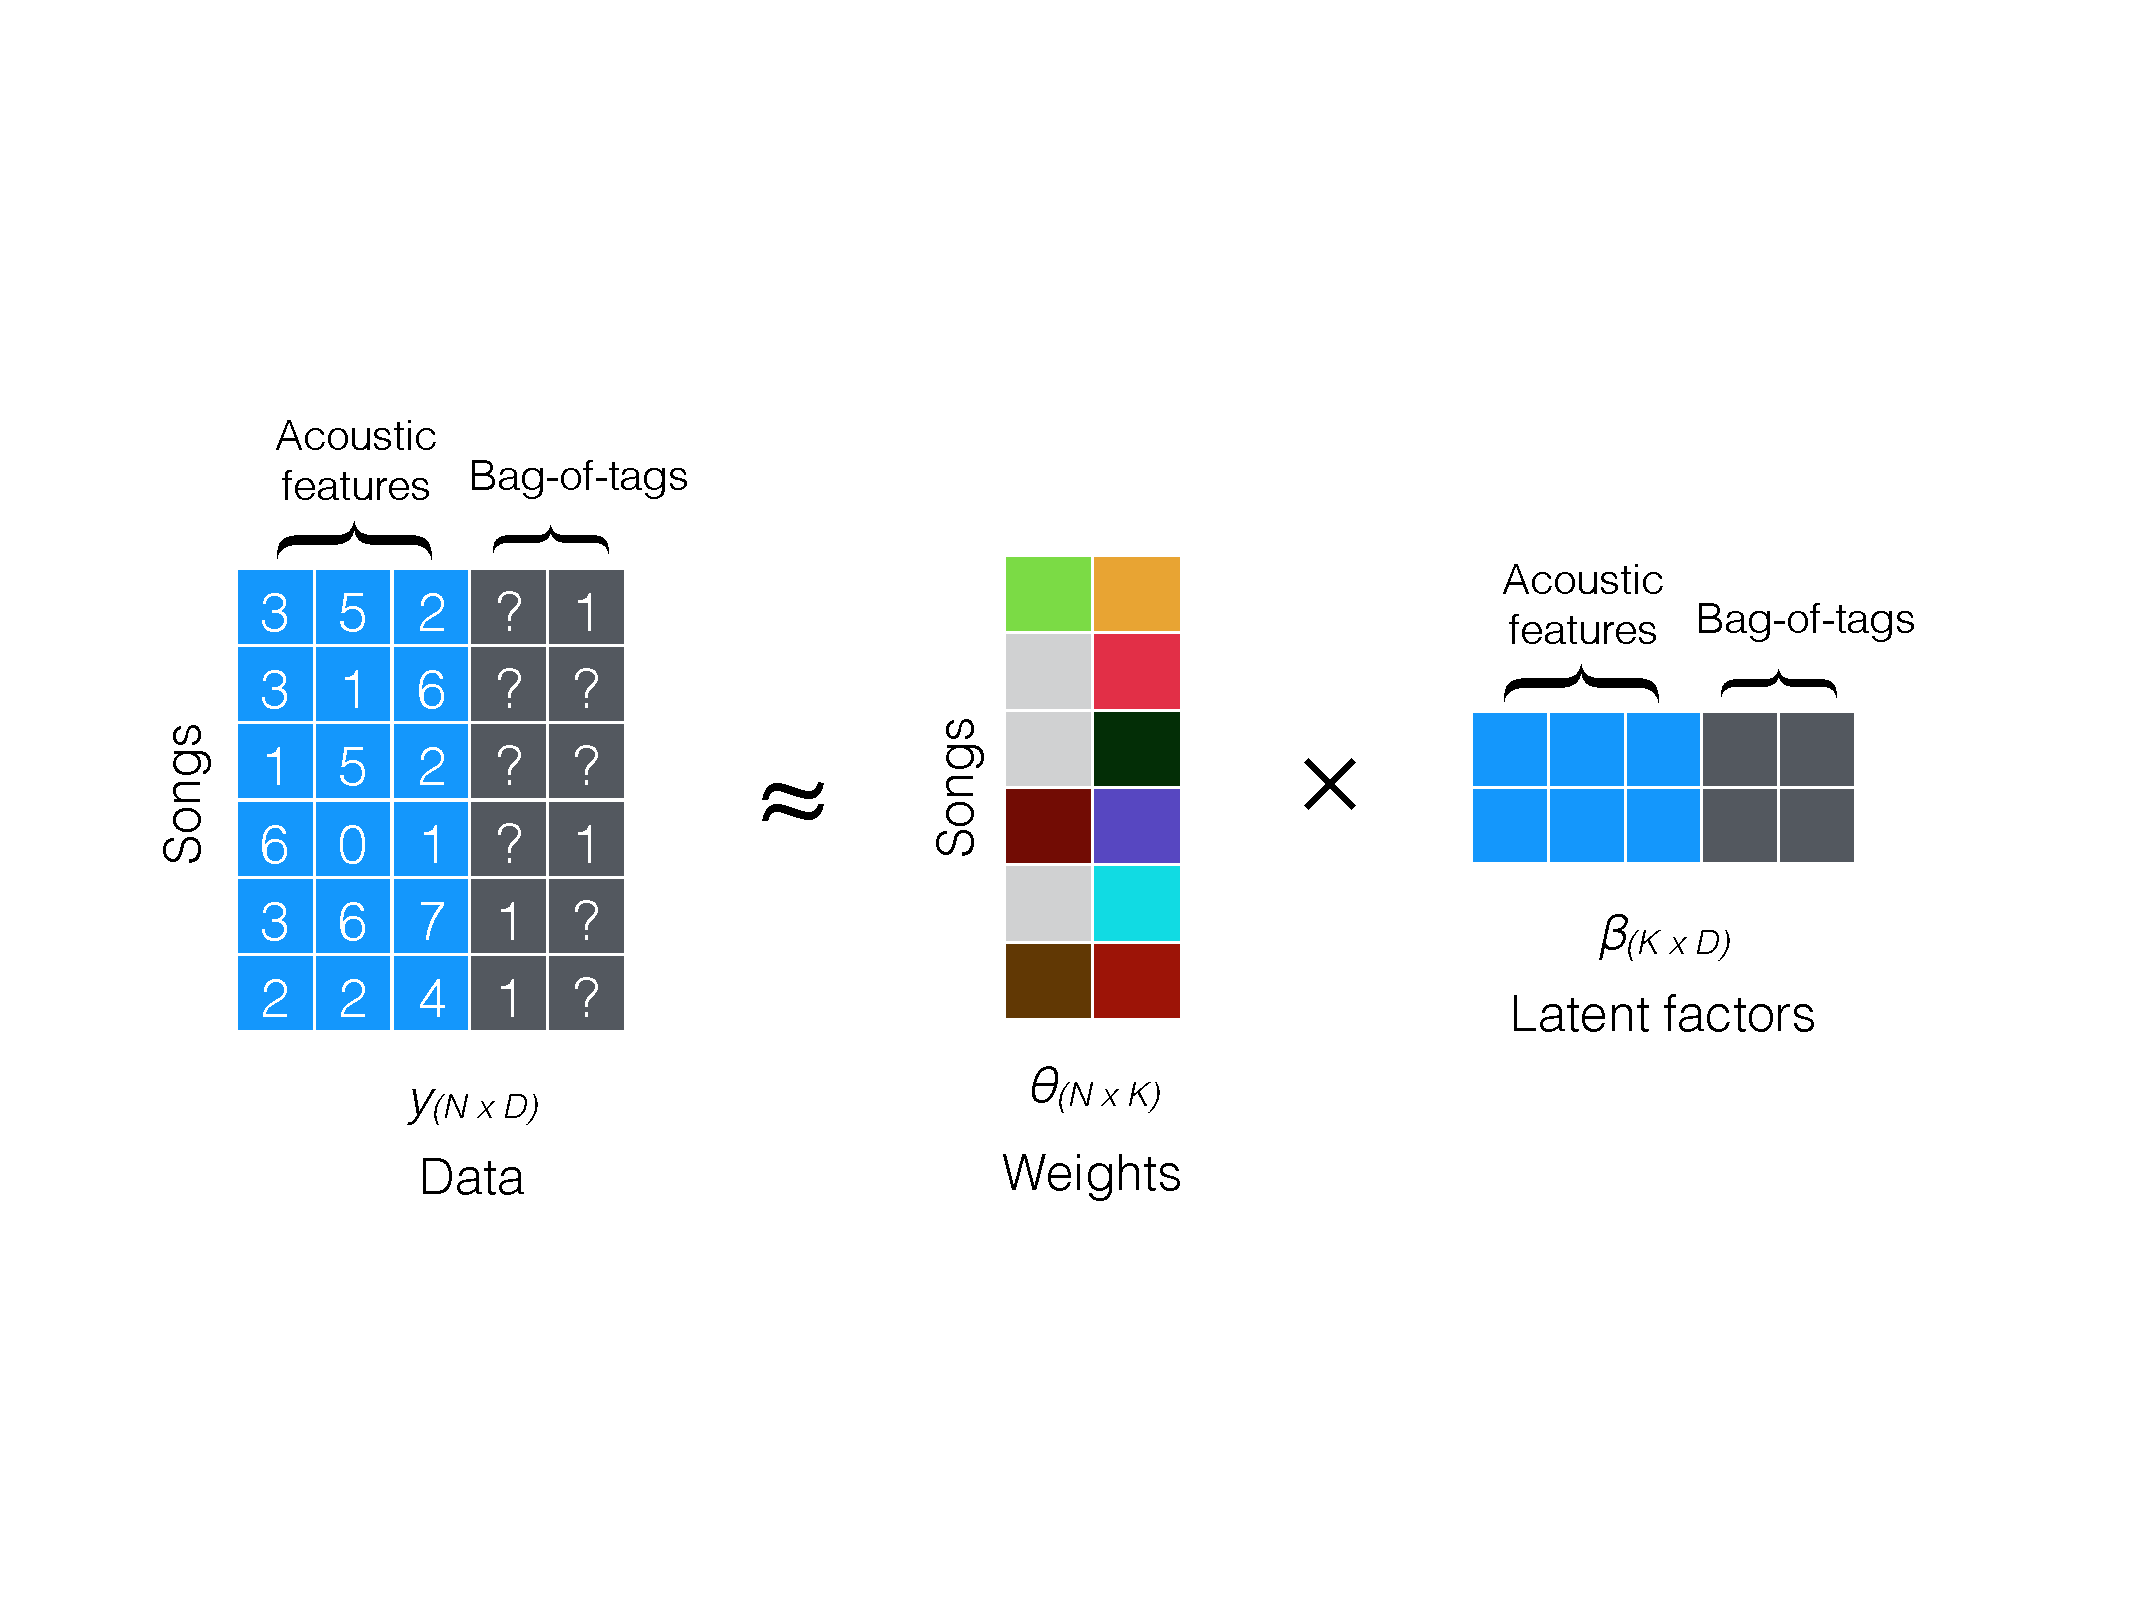
\includegraphics[width=\textwidth]{fig/pmf_tagging}
      \caption{The workflow of the proposed automatic tagging system. The data (left) consists of both acoustic features and bag-of-tags vectors. When we apply the matrix factorization model to this data, the latent factors we learn (rightmost) will exploit the shared latent structure between semantic tags and acoustic codewords.}
      \label{chpt:tagging:fig:cartoon}
\end{figure}

\section{Poisson matrix factorization}\label{chpt:tagging:sec:pmf}
We adopt the notational convention that bold letters (e.g. $\mb{y}, \mb{\theta}, \mb{\beta}$) denote matrices. $i \in \{1, \cdots, I\}$ is used to index songs. $d \in \{1, \cdots, D\}$ is used to index feature dimensions. $k \in \{1, \cdots, K\}$ is used to index latent factors from the matrix factorization model. Given the data $\mb{y}\in \mathbb{N}^{I\times D}$ as described in \Cref{chpt:tagging:sec:data}, the Poisson matrix factorization model is formulated as follows:
\begin{equation} \label{chpt:tagging:eq:model} 
\begin{split}
\theta_{ik} &\sim \gam(a, ac),\\
\beta_{kd} &\sim \gam(b, b),\\
y_{id} &\sim \pois( \sum_{k=1}^K \theta_{ik} \beta_{kd}),
\end{split}
\end{equation}
where $\beta_k \triangleq [\beta_{k1}, \dots, \beta_{kD}]^\top \in \mathbb{R}_+^{D}$ denote the $k$th latent factor and $\theta_i \triangleq [\theta_{i1}, \dots, \theta_{iK}]^\top \in \mathbb{R}_{+}^{K}$ denote the weights for song $i$. $a$ and $b$ are model hyperparameters. $c$ is a scalar on the weights that we tune to maximize the likelihood. A graphical model representation for the Poisson matrix factorization is shown in \Cref{chpt:background:fig:pmf}.

\begin{figure}[ht]
  \centering
     \begin{tikzpicture}

 % Define nodes
  \node[obs]                               (y) {$y_{id}$};
  \node[latent, above=of y, xshift=-1.2cm] (t) {$\theta_{ik}$};
  \node[latent, above=of y, xshift=1.2cm]  (b) {$\beta_{kd}$};


  % Connect the nodes
  \edge {b,t} {y} ; %

  % Plates
  \plate {tb} {(t)(b)} {$K$} ;
  \plate {yb} {(b)(y) (tb.north east)} {$D$} ;
  \plate {} {(t)(y) (tb.north west)(yb.north west)(yb.south west)} {$I$} ;

\end{tikzpicture}

  \caption{Graphical model representation for the Poisson matrix factorization.}
\label{chpt:background:fig:pmf}
\end{figure}

There are a couple of reasons to choose a Poisson model over a more traditional Gaussian model \citep{salakhutdinov2008probabilistic}. First, the Poisson distribution is a more natural choice to model count data. Secondly, real-world tagging data is extremely noisy and sparse. If a tag is not associated with a song in the data, it could be either because that tag does not apply to the song, or simply because no one has labeled the song with the tag yet. The Poisson matrix factorization model has the desirable property that it does not penalize values of $0$ as strongly as the Gaussian distribution \citep{paisley2015handbook,Gopalan:2015}. Therefore, even weakly labeled data can be used to learn the Poisson model.  

\section{Variational inference}

To learn the latent factors $\mb{\beta}$ and the corresponding decomposition weights $\mb{\theta}$ from the training data $\mb{y}$, we need to compute the posterior distribution $p(\mb{\theta}, \mb{\beta} | \mb{y})$. However, no closed-form expression exists for this hierarchical model. We therefore employ mean-field variational inference to approximate this posterior as described in \Cref{chpt:background:sec:vi}.

We choose a fully-factorized family of variational distributions,
\begin{equation*}
q(\mb{\theta}, \mb{\beta}) = \prod_{k=1}^K \Big(\prod_{i=1}^I q_{ik}(\theta_{ik})\Big) \Big(\prod_{d=1}^D q_{kd}(\beta_{kd})\Big),
\end{equation*}
to approximate the posterior $p(\mb{\theta}, \mb{\beta} | \mb{y})$, so that the
\gls{KL}-divergence between the variational distribution and
the true posterior is minimized. Following a further approximation discussed in the next section, the factorized distribution allows for a closed-form expression of this variational objective, and thus tractable inference. Here we choose variational distributions from the same family as the prior (we use the shape and rate parametrization for gamma distribution):
\begin{equation*}
\begin{split}
q_{ik}(\theta_{ik}) &= \gam(\theta_{ik}; \gamma_{ik}, \chi_{ik}),\\
q_{kd}(\beta_{kd}) &= \gam(\beta_{kd}; \nu_{kd},  \lambda_{kd}).
\end{split}
\end{equation*}
Minimizing the \gls{KL}-divergence is equivalent to maximizing the following variational objective (\gls{ELBO}):
\begin{align*}\label{eq:vlb}
\mathcal{L} =~& \EE{q}{\ln p(\mb{y}, \mb{\theta}, \mb{\beta})} + H(q),
\end{align*}
where $H(q)$ is the entropy of the variational distribution $q$.
We can optimize the variational objective using coordinate ascent via two approaches: batch inference, which requires processing of the entire dataset for every iteration; or stochastic inference, which only needs a small batch of data for each iteration and can be potentially scale to much larger datasets where batch inference is no longer computationally feasible.

\subsection{Batch inference} \label{chpt:tagging:sec:batch_vi}
Although the model in \Cref{chpt:tagging:eq:model} is not conditionally conjugate by itself, as demonstrated in \citet{cemgil2009bayesian}, we can introduce latent auxiliary random variables $z_{idk} \sim \text{Poisson}( \theta_{ik} \beta_{kd})$ ($y_{id} = \sum_k z_{idk}$)
with the variational distribution being $q(z_{idk}) = \mult(z_{id}; \phi_{id})$, where $z_{id} \in \mathbb{N}^K$, $\phi_{idk} \geq 0$ and $\sum_k \phi_{idk} = 1$.
This makes the model conditionally conjugate, which means that closed-form coordinate ascent updates are available. 

Following the standard results of variational inference for conditionally conjugate model (e.g. \cite{hoffman2013stochastic}), we can obtain the updates for $\theta_{ik}$:
\begin{equation}\label{chpt:background:eq:theta}
\begin{split}
\gamma_{ik} &= a + \sum_{d=1}^D y_{id} \phi_{idk},\\
\chi_{ik} &= ac + \sum_{d=1}^D \EE{q}{\beta_{kd}}.
\end{split}
\end{equation}
The scale $c$ is updated as:
\[
c^{-1} = \frac{1}{IK}\sum_{i, k} \mathbb{E}_q [\theta_{ik}].
\]

Similarly, we can obtain the updates for $\beta_{kd}$:
\begin{equation}\label{chpt:background:eq:beta}
\begin{split}
\nu_{kd} &= b + \sum_{i=1}^I y_{id} \phi_{idk},\\
\lambda_{kd} &= b + \sum_{i=1}^I \mathbb{E}_q[\theta_{ik}].
\end{split}
\end{equation}
Finally, for the auxiliary variables $z_{idk}$, the following update is applied:
\begin{equation*}
\phi_{idk} \propto \exp\{\mathbb{E}_q [\ln \theta_{ik} \beta_{kd}]\}.
\end{equation*}
Note that this update should be applied after either updating $\theta_{ik}$ or $\beta_{kd}$.
The necessary expectations for $\theta_{ik}$ are:
\begin{equation*}
\begin{split}
\mathbb{E}_q[\theta_{ik}] &= \gamma_{ik} / \chi_{ik}, \\
\mathbb{E}_q[\ln \theta_{ik}] &= \psi(\gamma_{ik}) - \ln \chi_{ik},
\end{split}
\end{equation*}
where $\psi(\cdot)$ is the digamma function. The expectations for $\beta_{kd}$ have the same form, but use $\nu_{kd}$ and $\lambda_{kd}$. The full algorithm of batch inference for the Poisson matrix factorization is summarized in \Cref{chpt:tagging:algo:batch_vi}.

\begin{algorithm}
\DontPrintSemicolon % Some LaTeX compilers require you to use \dontprintsemicolon instead 
\KwIn{Acoustic features and bag-of-tags vectors $\mby$, hyperparameters $a$ and $b$}
\KwOut{Variatioanl parameters $\mb\gamma$, $\mb\chi$, $\mb\nu$, $\mb\lambda$}
%$C \gets \emptyset$\;
Randomly initialize variational parameters $\mb\gamma$, $\mb\chi$, $\mb\nu$, $\mb\lambda$\;
\While{not converged}{
  \For{$(i, d): y_{id} > 0 $} {
  \For{$k \gets 1$ \textbf{to} $K$} {
   Update auxiliary variables $\phi_{idk}\propto \exp\{\mathbb{E}_q [\ln \theta_{ik} \beta_{kd}]\}$.
   }
  }
  \For{$i \gets 1$ \textbf{to} $I$}{
  \For{$k \gets 1$ \textbf{to} $K$}{
  	Update variational parameters $\gamma_{ik}$ and $\chi_{ik}$ for weights $\theta_{ik}$ (\Cref{chpt:background:eq:theta})
	}
	}
  Update scale $c^{-1} = \frac{1}{IK}\sum_{i, k} \mathbb{E}_q [\theta_{ik}]$\;
  \For{$(i, d): y_{id} > 0 $} {
  \For{$k \gets 1$ \textbf{to} $K$} {
   Update auxiliary variables $\phi_{idk}\propto \exp\{\mathbb{E}_q [\ln \theta_{ik} \beta_{kd}]\}$.
   }
  }
  \For{$d \gets 1$ \textbf{to} $D$}{
  \For{$k \gets 1$ \textbf{to} $K$}{
  	Update variational parameters $\nu_{kd}$ and $\lambda_{kd}$ for latent factors $\beta_{kd}$ (\Cref{chpt:background:eq:beta})
	}
	}
}
\Return{$\mb\gamma$, $\mb\chi$, $\mb\nu$, $\mb\lambda$}\;
\caption{{\sc BatchVI} Batch variational inference for the Poisson matrix factorization}
\label{chpt:tagging:algo:batch_vi}
\end{algorithm}

\subsection{Stochastic inference}\label{chpt:tagging:sec:svi}

Batch inference will alternate between updating $\mb{\theta}$ and $\mb{\beta}$ using the entire data at each iteration until convergence to a local optimum, which could be computationally intensive for large datasets. We can instead adopt stochastic optimization by selecting a subset (mini-batch) of the data at iteration $t$, indexed by $B_t \subset \{1, \cdots, I\}$, and optimizing over a noisy version of the variational objective $\mathcal{L}$:
\begin{equation}\label{chpt:tagging:eq:noisy_obj}
\cL_t = \frac{I}{|B_t|}\sum_{i \in B_t} \EE{q}{\ln p(y_i , \theta_i | \mb{\beta})}  + \EE{q}{\ln p(\mb{\beta})} + H(q).
\end{equation}
By optimizing $\cL_t$, we are optimizing $\cL$ in expectation. 

The updates for weights $\theta_{ik}$ and auxiliary variables $z_{idk}$ are essentially the same as those of batch inference, except that now we are only inferring weights for the mini-batch of data for $i \in B_t$. The optimal scale $c$ is updated accordingly:
\begin{equation*}
c^{-1} = \frac{1}{|B_t| K}\sum_{i \in B_t, k} \mathbb{E}_q [\theta_{ik}].
\end{equation*}

After alternating between updating weights $\theta_{ik}$ and latent variables $z_{idk}$ until convergence, we can take a gradient step,  preconditioned by the inverse Fisher information matrix of variational distribution $q_{kd}(\beta_{kd})$, to optimize $\beta_{kd}$ (see \cite{hoffman2013stochastic} for more technical details), 
\begin{equation*}
\begin{split}
\nu_{kd}^{(t)} &= (1 - \rho_t) \nu_{kd}^{(t-1)} + \rho_t \biggl(b +  \frac{I}{|B_t|}\sum_{i \in B_t} y_{id} \phi_{idk}\biggl),\\
\lambda_{kd}^{(t)} &= (1 - \rho_t) \lambda_{kd}^{(t-1)} + \rho_t \biggl( b +  \frac{I}{|B_t|}\sum_{i \in B_t} \mathbb{E}_q[\theta_{ik}]\biggl),
\end{split}
\end{equation*}
where $\rho_t > 0$ is a step size at iteration $t$. To ensure convergence \citep{bottou1998online}, the following conditions must be satisfied:
\begin{equation*}
\textstyle\sum_{t=1}^\infty\rho_t = \infty,\quad \sum_{t=1}^\infty \rho_t^2 < \infty.
\end{equation*}
One possible choice of $\rho_t$ is $\rho_t = (t_0 + t)^{-\kappa}$ for $t_0 > 0$ and $\kappa \in (0.5, 1]$. It has been shown \citep{hoffman2013stochastic} that this update corresponds to stochastic optimization with a natural gradient step, which better fits the geometry of the parameter space for probability distributions. The full algorithm for stochastic variational inference is summarized in \Cref{chpt:tagging:algo:svi}. Note that unlike \Cref{chpt:tagging:algo:batch_vi} where the variational parameters for weights $\mb\gamma$ and $\mb\chi$ are also returned, here we only return the learned variational parameters for latent factors $\mb\nu$ and $\mb\lambda$ to demonstrate the ``online'' natural of the stochastic variational inference algorithm: the data is processed in mini-batches and there is no need to keep track of any old data that has been already analyzed. 

\begin{algorithm}
\DontPrintSemicolon % Some LaTeX compilers require you to use \dontprintsemicolon instead 
\KwIn{Acoustic features and bag-of-tags vectors $\mby$, hyperparameters $a$, $b$, $t_0$, $\kappa$, and mini-batch size}
\KwOut{Variatioanl parameters $\mb\nu$, $\mb\lambda$}
%$C \gets \emptyset$\;
Randomly initialize variational parameters $\mb\nu$, $\mb\lambda$\;
\For{$t \gets 1,\dots$}{
  Subsample a mini-batch of data $B_t$\;
  \While{not converged}{
  \For{$(i, d): i \in B_t$ and $y_{id} > 0 $} {
  \For{$k \gets 1$ \textbf{to} $K$} {
   Update auxiliary variables $\phi_{idk}\propto \exp\{\mathbb{E}_q [\ln \theta_{ik} \beta_{kd}]\}$.
   }
  }
  \For{$i \in B_t$}{
  \For{$k \gets 1$ \textbf{to} $K$}{
  	Update variational parameters $\gamma_{ik}$ and $\chi_{ik}$ for weights $\theta_{ik}$ (\Cref{chpt:background:eq:theta})
	}
	}
  Update scale $c^{-1} = \frac{1}{|B_t| K}\sum_{i \in B_t, k} \mathbb{E}_q [\theta_{ik}]$\;
  }
  Set step size $\rho_t = (t_0 + t)^{-\kappa}$\;
  \For{$d \gets 1$ \textbf{to} $D$}{
  \For{$k \gets 1$ \textbf{to} $K$}{
  	Take natural gradient steps for latent factors:\;
  	$\qquad\nu_{kd}^{(t)} = (1 - \rho_t) \nu_{kd}^{(t-1)} + \rho_t \biggl(b +  \frac{I}{|B_t|}\sum_{i \in B_t} y_{id} \phi_{idk}\biggl)$\;
	$\qquad\lambda_{kd}^{(t)} = (1 - \rho_t) \lambda_{kd}^{(t-1)} + \rho_t \biggl( b +  \frac{I}{|B_t|}\sum_{i \in B_t} \mathbb{E}_q[\theta_{ik}]\biggl)$
	}
	}
}
\Return{$\mb\nu$, $\mb\lambda$}\;
\caption{{\sc SVI} Stochastic variational inference for the Poisson matrix factorization}
\label{chpt:tagging:algo:svi}
\end{algorithm}

\subsection{Generalizing to new songs}
Once the latent factor $\mb{\beta} \in \RR_+^{K \times D}$ is inferred, we can naturally divide it into two blocks: the VQ part $\mb{\beta}_{\text{VQ}} \in \mathbb{R}_+^{K \times J}$, and the bag-of-tags part $\mb{\beta}_{\text{BoT}} \in \RR_+^{K \times |V|}$. See the rightmost of \Cref{chpt:tagging:fig:cartoon} for an illustration.

Given a new song, we can first obtain the VQ feature $y_{\text{VQ}}$ and fit it with $\mb{\beta}_{\text{VQ}}$ to compute posterior of the weights $p(\theta | y_{\text{VQ}}, \mb{\beta}_{\text{VQ}})$. We can approximate this posterior with the variational inference algorithm in \Cref{chpt:tagging:sec:batch_vi} with $\mb{\beta}$ fixed. Then to predict tags, we can compute the expectation of the dot product between the weights $\theta$ and $\mb{\beta}_{\text{BoT}}$ under the variational distribution: 
\begin{equation} \label{chpt:tagging:eq:score}
\hat{y}_{\text{BoT}} = \EE{q}{\theta^T \mb{\beta}_{\text{BoT}}}.
\end{equation}
Since for different songs the weights $\theta$ may be scaled differently, before computing the dot product we normalize $\EE{q}{\theta}$ so that it lives on the probability simplex. To do automatic tagging, we could annotate the song with top $M$ tags according to $\hat{y}_{\text{BoT}}$. To compensate for a lack of diversity in the annotations, we adopt the same heuristic used in \cite{hoffman2009easy} by introducing a ``diversity factor'' $d$: For each predicted score, we subtract $d$ times the mean score for that tag. In our system, we set $d = 3$.

\section{Evaluation}\label{chpt:tagging:sec:exp}
We evaluate the model's performance on an annotation task and a retrieval task using CAL500 \citep{Turnbull_SemanticAudio} and Million Song Dataset (MSD) \citep{bertin2011million}. Unlike the CAL500 dataset where tracks are carefully-annotated, the Last.fm dataset associated with MSD comes from real-world user tagging, and thus contains only weakly labeled data with a tagging vocabulary that is much larger and more diverse.

We compare our results on these tasks with two other sets of codebook-based methods: Codeword Bernoulli Average (CBA) \citep{hoffman2009easy} and $\ell_2$-regularized logistic regression \citep{xie2011music}. Like the Poisson matrix factorization model, both methods are easy to train and can scale to relatively large dataset on a single machine. However, since both methods perform optimization in a batch fashion, we will later refer to them as ``batch algorithms'', along with the Poisson model with batch inference described in \Cref{chpt:tagging:sec:batch_vi}.

For the hyperparameters of the Poisson matrix factorization model, we set $a = b = 0.1$, and the number of latent factors $K = 100$. To learn the latent factors $\mb{\beta}$, we followed the procedure in \Cref{chpt:tagging:algo:batch_vi} for batch inference until the relative increase on the \gls{ELBO} is less than $0.05\%$. For stochastic inference, we followed the procedure in \Cref{chpt:tagging:algo:svi} and used a mini-batch size $|B_t| = 1,000$ unless otherwise specified and took a full pass of the randomly permuted data. As for the learning rate, we set $t_0 = 1$ and $\kappa = 0.6$. All the source code in Python is available online\footnote{\url{http://github.com/dawenl/stochastic_PMF}}.

\subsection{Annotation task}
The purpose of annotation task is to automatically tag unlabeled songs. To evaluate the model's ability for annotation, we computed the average per-tag precision, recall, and F-score on a test set. Per-tag precision is defined as the average fraction of songs that the model annotates with tag $v$ that are actually labeled $v$. Per-tag recall is defined as the average fraction of songs that are actually labeled $v$ that the model also annotates with tag $v$. F-score is the harmonic mean of precision and recall, and is one overall metric for annotation performance.

\subsection{Retrieval task}
The purpose of the retrieval task is, when given a query tag $v$, to provide a list of songs which are related to tag $v$. To evaluate the models' retrieval performance, for each tag in the vocabulary we ranked each song in the test set by the predicted score from \Cref{chpt:tagging:eq:score}. We evaluated the area under the receiver-operator curve (AROC) and mean average precision (MAP) for each ranking. AROC is defined as the area under the curve, which plots the true positive rate against the false positive rate, and MAP is defined as the mean of the average precision (AP) for each tag, which is the average of the precisions at each possible level of recall. 

\subsection{Results on CAL500}
Following the procedure similar to that described in \citet{hoffman2009easy,xie2011music}, we performed a 5-fold cross-validation to evaluate the annotation and retrieval performance on CAL500. We selected the top 78 tags, which are annotated more than 50 times in the dataset, and learned a codebook of size $J = 2000$. For the annotation task, we labeled each song with the top 10 tags based on the predicted score. Since CAL500 is a relatively small dataset, we only performed batch inference for the Poisson matrix factorization model.

The results are reported in \Cref{tab:cal500}, which shows that the Poisson model has comparable performance on the annotation task, and does slightly worse on the retrieval task. As mentioned in \Cref{chpt:tagging:sec:pmf}, the Poisson matrix factorization model is particularly suitable for noisy and sparse data where $0$'s are not necessarily interpreted as explicit observations. However, this may not be the case for CAL500, as the vocabulary was well-chosen and the data was collected from a survey where the tagging quality is understandably higher than the actual tagging data in the real world, like the one from Last.fm. Therefore, this task cannot fully exploit the advantage brought by the Poisson model. 
Meanwhile, the amount of data in CAL500 is fairly small -- the data $\mb{y}$ fit to the model is simply a 502-by-2078 matrix. This prevents us from adopting stochastic inference, which will be shown being much more effective than batch inference even on a 10,000-song dataset in \Cref{chpt:tagging:sec:msd}. 

\begin{table}
\centering
  \begin{tabular}{ c  c  c  c  c  c }
    \toprule
    Model & Prec & Recall & F-score & AROC & MAP \\ \midrule
      CBA &  0.41 & 0.24    &   0.29    &   0.69  & 0.47 \\
     $\ell_2$ LogRegr & 0.48  &  0.26  & 0.34  &  0.72 & 0.50\\
    PMF-Batch & 0.42  &  0.23 & 0.30 & 0.67 & 0.45 \\
    \bottomrule
  \end{tabular}
  \caption{Results for the top 78 popular tags on CAL500, for Codeword Bernoulli Average (CBA), $\ell_2$ regularized logistic regression ($\ell_2$ LogRegr), and Poisson matrix factorization with batch inference (PMF-Batch). The results for CBA and $\ell_2$ LogRegr are directly copied from \cite{xie2011music}.} 
  \label{tab:cal500}
\end{table}


\subsection{Results on MSD}\label{chpt:tagging:sec:msd}
To demonstrate the scalability of the Poisson matrix factorization model, we conducted experiments using MSD and the associated Last.fm dataset. To our knowledge, there has not been any previous work where music tagging results are reported on the MSD. 

Since the Last.fm dataset contains 522,366 unique tags, it is not realistic to build the model with all of them. We first selected the tags with more than 1,000 appearances and removed those which do not carry discriminative information (e.g. ``my favorite'', ``awesome'', ``seen live'', etc.). Then we ran the stemming algorithm implemented in \emph{NLTK}\footnote{\url{http://www.nltk.org/}} to further reduce the potential duplications and correct for alternate spellings (e.g. ``pop-rock'' v.s. ``pop rock'', ``love song'' v.s. ``love songs''), which gave us a vocabulary of 561 tags. Using the default train/test artist split from MSD, we filtered out the songs which have been labeled with tags from the selected vocabulary. This gave us 371,209 songs for training. For test set, we further selected those which have at least 20 tags (otherwise, it is likely that this song is very weakly labeled). This gave us a test set of 2,757 songs. The feature we used is the Echo Nest's timbre feature, which is very similar to MFCC. 

We randomly selected 10,000 songs as the data which can fit into the memory nicely for all the batch algorithms, and trained the following models with different codebook sizes $J \in \{256, 512, 1024, 2048 \}$: Codeword Bernoulli Average (CBA), $\ell_2$-regularized logistic regression ($\ell_2$ LogRegr), Poisson matrix factorization with batch inference (PMF-Batch) and stochastic inference by a single pass of the data (PMF-Stoc-$10K$). Here we used batch size $|B_t| = 500$ for PMF-Stoc-$10K$, as otherwise there will only be 10 mini-batches from the subset. However, given enough data, in general larger batch size will lead to relatively superior performance, since the variance of the noisy variational objective in \Cref{chpt:tagging:eq:noisy_obj} is smaller. To demonstrate the effectiveness of the Poisson model on massive amount of data (exploiting the stochastic algorithm's ability to run without loading the entire dataset into memory), we also trained the model with the full training set with stochastic 
inference (PMF-Stoc-full). For the annotation task, we labeled each song with the top 20 tags based on the predicted score. 

The results are reported in \Cref{chpt:tagging:tab:msd}. In general, the performance of Poisson matrix factorization is comparably better for smaller codebook size $J$. Specifically, for stochastic inference, even if the amount of training data is relatively small,  it is not only significantly faster than batch inference, but can also help improve the performance by quite a large margin. Finally, not surprisingly, PMF-Stoc-full dominates all the metrics, regardless of the size of the codebook, because it is able to learn from more data. 


\begin{sidewaystable}
\centering 
%\small
\begin{tabular}{  c    c   c  c  c  c  c }
\toprule
Codebook size & Model & Precision & Recall & F-score & AROC & MAP  \\
\midrule
 \multicolumn{1}{ c }{\multirow{5}{*}{$J=256$} }& CBA & 0.112 (0.007) & 0.121 (0.008) &0.116	& 0.695 (0.005) &  0.112 (0.006) \\
 \multicolumn{1}{c}{} & $\ell_2$ LogRegr & 0.091 (0.008) &	0.093 (0.006)	&0.092	&0.692 (0.005)	& 0.110 (0.006)\\
  \multicolumn{1}{c}{}  & PMF-Batch & 0.113 (0.007) & 0.105 (0.006)	 & 0.109 &	0.647 (0.005)	& 0.094 (0.005) \\
    \multicolumn{1}{c}{}  & PMF-Stoc-$10K$ & 0.116 (0.007) & 0.127 (0.007) & 0.121 & 0.682 (0.005) & 0.105 (0.006) \\
    \multicolumn{1}{c}{}  & PMF-Stoc-full & \bf 0.127 (0.008) &  \bf 0.143 (0.008)	 & \bf 0.134 & \bf 0.704 (0.005) & \bf 0.115 (0.006) \\ 
   
    \midrule
 \multicolumn{1}{ c }{\multirow{5}{*}{$J=512$} }& CBA & 0.120 (0.007)&0.127 (0.008)&0.124&0.689 (0.005) & 0.117 (0.006) \\
 \multicolumn{1}{c}{} & $\ell_2$ LogRegr & 0.096 (0.008)	& 0.108 (0.007) & 	0.101 &	0.693 (0.005)	& 0.113 (0.006)\\
  \multicolumn{1}{c}{}  & PMF-Batch & 0.111 (0.007)	& 0.108 (0.006)	&0.109&	0.645 (0.005)&	0.098 (0.005) \\
    \multicolumn{1}{c}{}  & PMF-Stoc-$10K$ & 0.112 (0.007) &0.128 (0.007) & 0.120 &  0.687 (0.005) & 0.110 (0.006)\\
    \multicolumn{1}{c}{}  & PMF-Stoc-full & \bf0.130 (0.008)& \bf 0.154 (0.008) & \bf 0.141 & \bf 0.715 (0.005) & \bf 0.122 (0.006) \\ 
    
    \midrule
 \multicolumn{1}{ c }{\multirow{5}{*}{$J=1024$} }& CBA & 0.118 (0.007)&0.126 (0.007)&0.122&0.692 (0.005)&0.117 (0.006) \\
 \multicolumn{1}{c}{} & $\ell_2$ LogRegr &  0.113 (0.008)&0.129 (0.008)&0.120&0.698 (0.005)&0.115 (0.006\\
  \multicolumn{1}{c}{}  & PMF-Batch & 0.112 (0.007)	& 0.109 (0.006)	& 0.111 & 0.635 (0.005) & 0.098 (0.006) \\
    \multicolumn{1}{c}{}  & PMF-Stoc-$10K$ & 0.111 (0.007) & 0.127 (0.007) & 0.118 & 0.687 (0.005) & 0.111 (0.006) \\
    \multicolumn{1}{c}{}  & PMF-Stoc-full & \bf 0.127 (0.008) & \bf 0.146 (0.008) & \bf 0.136 & \bf 0.712 (0.005) & \bf 0.120 (0.006)\\ 
    
        
    \midrule
 \multicolumn{1}{ c }{\multirow{5}{*}{$J=2048$} }& CBA &\bf 0.124 (0.007) & 0.129 (0.007) &0.127 &0.689 (0.005) & 0.117 (0.006) \\
 \multicolumn{1}{c}{} & $\ell_2$ LogRegr & 0.115 (0.008) & 0.137 (0.008)	& 0.125 &0.698 (0.005) & \bf 0.118 (0.006)\\
  \multicolumn{1}{c}{}  & PMF-Batch & 0.109 (0.007) & 0.110 (0.006) & 0.110 & 0.637 (0.005)	&0.098 (0.006) \\
    \multicolumn{1}{c}{}  & PMF-Stoc-$10K$ & 0.107 (0.007) & 0.124 (0.007) & 0.115 & 0.682 (0.005) & 0.106 (0.006) \\
    \multicolumn{1}{c}{}  & PMF-Stoc-full & 0.120 (0.007) & \bf 0.147 (0.008)	 & \bf 0.132 & \bf 0.712 (0.005) & \bf 0.118 (0.006) \\\bottomrule 
    
\end{tabular}  
\caption{ Annotation (evaluated using precision, recall, and F-score) and retrieval (evaluated using area under the receiver-operator curve (AROC) and mean average precision (MAP)) performance on the Million Song Dataset with various codebook sizes, from Codeword Bernoulli Average (CBA), $\ell_2$ regularized logistic regression ($\ell_2$ LogRegr), Poisson matrix factorization with batch inference (PMF-Batch) and stochastic inference by a single pass of the subset (PMF-Stoc-$10K$) and full data (PMF-Stoc-full). One standard error is reported in the parenthesis. }
\label{chpt:tagging:tab:msd}
\end{sidewaystable} 

\begin{figure}
  \centering
    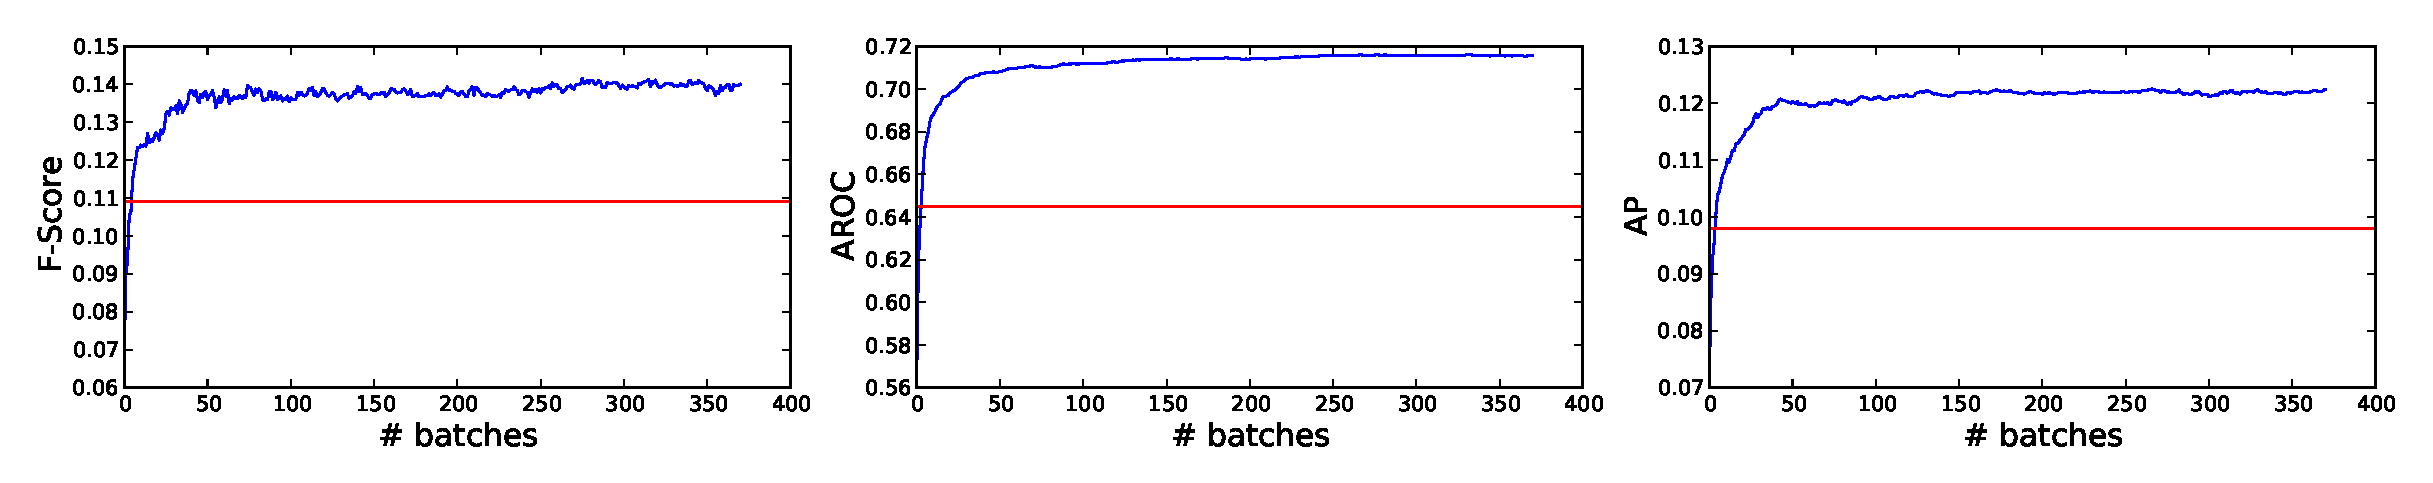
\includegraphics[width=.98\textwidth]{fig/metrics_K512}
      \caption{Improvement in performance with the number of mini-batches consumed for the PMF-Stoc-full system with $J=512$.  Red lines indicate the performance of PMF-Batch which is trained on 10k 
      examples; that system's performance is exceeded after fewer than 5 mini-batches.}
      \label{fig:performance}
\end{figure}

\Cref{fig:performance} illustrates how the metrics improve as more data becomes available for the Poisson matrix factorization model, showing how the F-score, AROC, and MAP improve with the number of (1000-element) mini-batches consumed up to the entire 371k training set.  We see that initial growth is rapid, thanks to the natural gradient, with much of the benefit obtained after just 50 batches.  However, we see continued improvement beyond this; it is reasonable to believe that if more data becomes available, the performance can be further improved. On the other hand, we also observe that the performance is limited by the modeling capacity of a (bi-)linear factorization model. In \Cref{chpt:content}, we show that superior performance can be achieved with a deep neural net. 

\Cref{tab:factors} contains information on the qualitative performance of our model. The tagging model works by capturing correlations between semantic tags and acoustic codewords in each latent factor $\beta_k$. As discussed, when a new song arrives with missing tag information, only the portion of $\beta_k$ corresponding to acoustic codewords is used, and the semantic tag portion of $\beta_k$ is used to make predictions of the missing tags. Similar to related topic models \citep{hoffman2013stochastic}, we can therefore look at the highly probable tags for each $\beta_k$ to understand what portion of the acoustic codeword space is being captured by that factor, and whether it is musically coherent. We show an example of this in \Cref{tab:factors}, where we list the top 7 tags from 9 latent factors $\beta_k$ learned by our model with $J=512$. We sort the tags according to expected relevance under the variational distribution $\EE{q}{\beta_{kd}}$. This shows which tags are considered to have 
high probability for a song that has the given factor expressed. As is evident, each factor corresponds to a particular aspect of a music genre. We note that other factors contained similarly coherent tag information.


\begin{sidewaystable}
\footnotesize
\centering
\begin{tabular}{ ccccccccc }
\toprule
\hspace{-6pt}\emph{``Pop''} &  \emph{``Indie''} &  \emph{``Jazz''} & \emph{``Classical''} & \emph{``Metal''} & \emph{``Reggae''} & \emph{``Electronic''} & \emph{``Experimental''} & \emph{``Country''} \hspace{-6pt}\\
\hline
\hspace{-6pt}pop & indie & chillout & piano & metal & reggae & house & instrumental  & country\hspace{-6pt}\\ 
\hspace{-6pt}female vocal & rock & lounge & instrumental & death metal  & funk & electro & ambient & classic country\hspace{-6pt} \\ 
\hspace{-6pt}dance & alternative & chill & ambient & thrash metal  & funky & electronic & experimental & male vocal\hspace{-6pt} \\ 
\hspace{-6pt}electronic & indie rock & downtempo & classic & brutal death metal  & dance & dance & electronic & blues\hspace{-6pt}\\ 
\hspace{-6pt}sexy & post punk & smooth jazz & beautiful & grindcore  & hip-hop & electric house & psychedelic & folk\hspace{-6pt} \\ 
\hspace{-6pt}love & psychedelic & relax & chillout & heavy metal  & party & techno & progressive & love songs\hspace{-6pt}\\
\hspace{-6pt}synth pop & new wave & ambient & relax & black metal & sexy & minimal & rock & americana \hspace{-6pt}\\
\bottomrule
\end{tabular}
\caption{Top 7 tags from 9 latent factors for PMF-Stoc-full with $J=512$. For each factor, we assign the closest music genre on top. As is evident, each factor corresponds to a particular aspect of a music genre.}\label{tab:factors}
\normalsize
\end{sidewaystable}


\section{Summary}\label{sec:conclusion}
We present a codebook-based scalable music tagging model with Poisson matrix factorization. 
The system learns the joint behavior of acoustic features and semantic tags, which can be used to infer 
the most appropriate tags given the audio alone.  The Poisson model is naturally less sensitive to 
zero values than some alternatives, making it a good match to ``noisy'' training examples derived from 
real users' taggings, where the fact that no user has applied a tag does not necessarily imply that the term is irrelevant.  By learning this model using stochastic variational inference, we are able to efficiently 
exploit much larger training sets than are tractable using batch approaches, making it feasible to learn 
from an entire set of over 370k tagged examples.  Although much of the improvement comes in the earlier iterations, we see continued improvement implying this approach can benefit from much larger, effectively unlimited sources of tagged examples, as might be available on a commercial music service with millions of users.

There are a few areas where our model can be easily developed. For example, stochastic variational inference requires we set the learning rate parameters $t_0$ and $\kappa$, which is application-dependent. By using adaptive learning rates for stochastic variational inference \citep{ranganath2013adaptive}, model inference can converge faster and to a better local optimal solution. From a modeling perspective, currently the hyperparameters for weights $\mb{\theta}$ are fixed, indicating that the sparsity level of the weight for each song is assumed to be the same \emph{a priori}. Alternatively we could put \emph{song-dependent} hyper-priors on the hyperparameters of $\mb{\theta}$ to encode the intuition that some of the songs might have denser weights because more tagging information is available. This would offer more flexibility to the current model. 



%\bibliography{ismir2014}



